
%%%%%%%%%%%%%%%%%% PREAMBULE %%%%%%%%%%%%%%%%%%

\documentclass[aspectratio=169,utf8]{beamer}
%\documentclass[aspectratio=169,handout]{beamer}

\usetheme{Boadilla}
%\usecolortheme{seahorse}
\usecolortheme[RGB={245,66,24}]{structure}
\useoutertheme{infolines}

% packages
\usepackage{amsfonts,amsmath,amssymb,amsthm}
\usepackage[utf8]{inputenc}
\usepackage[T1]{fontenc}
\usepackage{lmodern}

\usepackage[francais]{babel}
\usepackage{fancybox}
\usepackage{graphicx}

\usepackage{float}
\usepackage{xfrac}

%\usepackage[usenames, x11names]{xcolor}
\usepackage{tikz}
\usepackage{pgfplots}
\usepackage{datetime}



%-----  Package unités -----
\usepackage{siunitx}
\sisetup{locale = FR,detect-all,per-mode = symbol}

%\usepackage{mathptmx}
%\usepackage{fouriernc}
%\usepackage{newcent}
%\usepackage[mathcal,mathbf]{euler}

%\usepackage{palatino}
%\usepackage{newcent}
% \usepackage[mathcal,mathbf]{euler}



% \usepackage{hyperref}
% \hypersetup{colorlinks=true, linkcolor=blue, urlcolor=blue,
% pdftitle={Exo7 - Exercices de mathématiques}, pdfauthor={Exo7}}


%section
% \usepackage{sectsty}
% \allsectionsfont{\bf}
%\sectionfont{\color{Tomato3}\upshape\selectfont}
%\subsectionfont{\color{Tomato4}\upshape\selectfont}

%----- Ensembles : entiers, reels, complexes -----
\newcommand{\Nn}{\mathbb{N}} \newcommand{\N}{\mathbb{N}}
\newcommand{\Zz}{\mathbb{Z}} \newcommand{\Z}{\mathbb{Z}}
\newcommand{\Qq}{\mathbb{Q}} \newcommand{\Q}{\mathbb{Q}}
\newcommand{\Rr}{\mathbb{R}} \newcommand{\R}{\mathbb{R}}
\newcommand{\Cc}{\mathbb{C}} 
\newcommand{\Kk}{\mathbb{K}} \newcommand{\K}{\mathbb{K}}

%----- Modifications de symboles -----
\renewcommand{\epsilon}{\varepsilon}
\renewcommand{\Re}{\mathop{\text{Re}}\nolimits}
\renewcommand{\Im}{\mathop{\text{Im}}\nolimits}
%\newcommand{\llbracket}{\left[\kern-0.15em\left[}
%\newcommand{\rrbracket}{\right]\kern-0.15em\right]}

\renewcommand{\ge}{\geqslant}
\renewcommand{\geq}{\geqslant}
\renewcommand{\le}{\leqslant}
\renewcommand{\leq}{\leqslant}
\renewcommand{\epsilon}{\varepsilon}

%----- Fonctions usuelles -----
\newcommand{\ch}{\mathop{\text{ch}}\nolimits}
\newcommand{\sh}{\mathop{\text{sh}}\nolimits}
\renewcommand{\tanh}{\mathop{\text{th}}\nolimits}
\newcommand{\cotan}{\mathop{\text{cotan}}\nolimits}
\newcommand{\Arcsin}{\mathop{\text{arcsin}}\nolimits}
\newcommand{\Arccos}{\mathop{\text{arccos}}\nolimits}
\newcommand{\Arctan}{\mathop{\text{arctan}}\nolimits}
\newcommand{\Argsh}{\mathop{\text{argsh}}\nolimits}
\newcommand{\Argch}{\mathop{\text{argch}}\nolimits}
\newcommand{\Argth}{\mathop{\text{argth}}\nolimits}
\newcommand{\pgcd}{\mathop{\text{pgcd}}\nolimits} 


%----- Commandes divers ------
\newcommand{\ii}{\mathrm{i}}
\newcommand{\dd}{\text{d}}
\newcommand{\id}{\mathop{\text{id}}\nolimits}
\newcommand{\Ker}{\mathop{\text{Ker}}\nolimits}
\newcommand{\Card}{\mathop{\text{Card}}\nolimits}
\newcommand{\Vect}{\mathop{\text{Vect}}\nolimits}
\newcommand{\Mat}{\mathop{\text{Mat}}\nolimits}
\newcommand{\rg}{\mathop{\text{rg}}\nolimits}
\newcommand{\tr}{\mathop{\text{tr}}\nolimits}


%----- Structure des exercices ------

\newtheoremstyle{styleexo}% name
{2ex}% Space above
{3ex}% Space below
{}% Body font
{}% Indent amount 1
{\bfseries} % Theorem head font
{}% Punctuation after theorem head
{\newline}% Space after theorem head 2
{}% Theorem head spec (can be left empty, meaning ‘normal’)

%\theoremstyle{styleexo}
\newtheorem{exo}{Exercice}
\newtheorem{ind}{Indications}
\newtheorem{cor}{Correction}


\newcommand{\exercice}[1]{} \newcommand{\finexercice}{}
%\newcommand{\exercice}[1]{{\tiny\texttt{#1}}\vspace{-2ex}} % pour afficher le numero absolu, l'auteur...
\newcommand{\enonce}{\begin{exo}} \newcommand{\finenonce}{\end{exo}}
\newcommand{\indication}{\begin{ind}} \newcommand{\finindication}{\end{ind}}
\newcommand{\correction}{\begin{cor}} \newcommand{\fincorrection}{\end{cor}}

\newcommand{\noindication}{\stepcounter{ind}}
\newcommand{\nocorrection}{\stepcounter{cor}}

\newcommand{\fiche}[1]{} \newcommand{\finfiche}{}
\newcommand{\titre}[1]{\centerline{\large \bf #1}}
\newcommand{\addcommand}[1]{}
\newcommand{\video}[1]{}

% Marge
\newcommand{\mymargin}[1]{\marginpar{{\small #1}}}

\def\noqed{\renewcommand{\qedsymbol}{}}


%----- Presentation ------
\setlength{\parindent}{0cm}

%\newcommand{\ExoSept}{\href{http://exo7.emath.fr}{\textbf{\textsf{Exo7}}}}

\definecolor{myred}{rgb}{0.93,0.26,0}
\definecolor{myorange}{rgb}{0.97,0.58,0}
\definecolor{myyellow}{rgb}{1,0.86,0}

\newcommand{\LogoExoSept}[1]{  % input : echelle
{\usefont{U}{cmss}{bx}{n}
\begin{tikzpicture}[scale=0.1*#1,transform shape]
  \fill[color=myorange] (0,0)--(4,0)--(4,-4)--(0,-4)--cycle;
  \fill[color=myred] (0,0)--(0,3)--(-3,3)--(-3,0)--cycle;
  \fill[color=myyellow] (4,0)--(7,4)--(3,7)--(0,3)--cycle;
  \node[scale=5] at (3.5,3.5) {Exo7};
\end{tikzpicture}}
}


\newcommand{\debutmontitre}{
  \author{} \date{} 
  \thispagestyle{empty}
  \hspace*{-10ex}
  \begin{minipage}{\textwidth}
    \titlepage  
  \vspace*{-2.5cm}
  \begin{center}
    \LogoExoSept{2.5}
  \end{center}
  \end{minipage}

  \vspace*{-0cm}
  
  % Astuce pour que le background ne soit pas discrétisé lors de la conversion pdf -> png
\begin{tikzpicture}
        \fill[opacity=0,green!60!black] (0,0)--++(0,0)--++(0,0)--++(0,0)--cycle; 
\end{tikzpicture}

% toc S'affiche trop tot :
% \tableofcontents[hideallsubsections, pausesections]
}

\newcommand{\finmontitre}{
  \end{frame}
  \setcounter{framenumber}{0}
} % ne marche pas pour une raison obscure

%----- Commandes supplementaires ------

% \usepackage[landscape]{geometry}
% \geometry{top=1cm, bottom=3cm, left=2cm, right=10cm, marginparsep=1cm
% }
% \usepackage[a4paper]{geometry}
% \geometry{top=2cm, bottom=2cm, left=2cm, right=2cm, marginparsep=1cm
% }

%\usepackage{standalone}


% New command Arnaud -- november 2011
\setbeamersize{text margin left=24ex}
% si vous modifier cette valeur il faut aussi
% modifier le decalage du titre pour compenser
% (ex : ici =+10ex, titre =-5ex

\theoremstyle{definition}
%\newtheorem{proposition}{Proposition}
%\newtheorem{exemple}{Exemple}
%\newtheorem{theoreme}{Théorème}
%\newtheorem{lemme}{Lemme}
%\newtheorem{corollaire}{Corollaire}
%\newtheorem*{remarque*}{Remarque}
%\newtheorem*{miniexercice}{Mini-exercices}
%\newtheorem{definition}{Définition}

% Commande tikz
\usetikzlibrary{calc}
\usetikzlibrary{patterns,arrows}
\usetikzlibrary{matrix}
\usetikzlibrary{fadings} 

%definition d'un terme
\newcommand{\defi}[1]{{\color{myorange}\textbf{\emph{#1}}}}
\newcommand{\evidence}[1]{{\color{blue}\textbf{\emph{#1}}}}
\newcommand{\assertion}[1]{\emph{\og#1\fg}}  % pour chapitre logique
%\renewcommand{\contentsname}{Sommaire}
\renewcommand{\contentsname}{}
\setcounter{tocdepth}{2}



%------ Figures ------

\def\myscale{1} % par défaut 
\newcommand{\myfigure}[2]{  % entrée : echelle, fichier figure
\def\myscale{#1}
\begin{center}
\footnotesize
{#2}
\end{center}}


%------ Encadrement ------

\usepackage{fancybox}


\newcommand{\mybox}[1]{
\setlength{\fboxsep}{7pt}
\begin{center}
\shadowbox{#1}
\end{center}}

\newcommand{\myboxinline}[1]{
\setlength{\fboxsep}{5pt}
\raisebox{-10pt}{
\shadowbox{#1}
}
}

%--------------- Commande beamer---------------
\newcommand{\beameronly}[1]{#1} % permet de mettre des pause dans beamer pas dans poly


\setbeamertemplate{navigation symbols}{}
\setbeamertemplate{footline}  % tiré du fichier beamerouterinfolines.sty
{
  \leavevmode%
  \hbox{%
  \begin{beamercolorbox}[wd=.333333\paperwidth,ht=2.25ex,dp=1ex,center]{author in head/foot}%
    % \usebeamerfont{author in head/foot}\insertshortauthor%~~(\insertshortinstitute)
    \usebeamerfont{section in head/foot}{\bf\insertshorttitle}
  \end{beamercolorbox}%
  \begin{beamercolorbox}[wd=.333333\paperwidth,ht=2.25ex,dp=1ex,center]{title in head/foot}%
    \usebeamerfont{section in head/foot}{\bf\insertsectionhead}
  \end{beamercolorbox}%
  \begin{beamercolorbox}[wd=.333333\paperwidth,ht=2.25ex,dp=1ex,right]{date in head/foot}%
    % \usebeamerfont{date in head/foot}\insertshortdate{}\hspace*{2em}
    \insertframenumber{} / \inserttotalframenumber\hspace*{2ex} 
  \end{beamercolorbox}}%
  \vskip0pt%
}


\definecolor{mygrey}{rgb}{0.5,0.5,0.5}
\setlength{\parindent}{0cm}
%\DeclareTextFontCommand{\helvetica}{\fontfamily{phv}\selectfont}

% background beamer
\definecolor{couleurhaut}{rgb}{0.85,0.9,1}  % creme
\definecolor{couleurmilieu}{rgb}{1,1,1}  % vert pale
\definecolor{couleurbas}{rgb}{0.85,0.9,1}  % blanc
\setbeamertemplate{background canvas}[vertical shading]%
[top=couleurhaut,middle=couleurmilieu,midpoint=0.4,bottom=couleurbas] 
%[top=fondtitre!05,bottom=fondtitre!60]



\makeatletter
\setbeamertemplate{theorem begin}
{%
  \begin{\inserttheoremblockenv}
  {%
    \inserttheoremheadfont
    \inserttheoremname
    \inserttheoremnumber
    \ifx\inserttheoremaddition\@empty\else\ (\inserttheoremaddition)\fi%
    \inserttheorempunctuation
  }%
}
\setbeamertemplate{theorem end}{\end{\inserttheoremblockenv}}

\newenvironment{theoreme}[1][]{%
   \setbeamercolor{block title}{fg=structure,bg=structure!40}
   \setbeamercolor{block body}{fg=black,bg=structure!10}
   \begin{block}{{\bf Th\'eor\`eme }#1}
}{%
   \end{block}%
}


\newenvironment{proposition}[1][]{%
   \setbeamercolor{block title}{fg=structure,bg=structure!40}
   \setbeamercolor{block body}{fg=black,bg=structure!10}
   \begin{block}{{\bf Proposition }#1}
}{%
   \end{block}%
}

\newenvironment{corollaire}[1][]{%
   \setbeamercolor{block title}{fg=structure,bg=structure!40}
   \setbeamercolor{block body}{fg=black,bg=structure!10}
   \begin{block}{{\bf Corollaire }#1}
}{%
   \end{block}%
}

\newenvironment{mydefinition}[1][]{%
   \setbeamercolor{block title}{fg=structure,bg=structure!40}
   \setbeamercolor{block body}{fg=black,bg=structure!10}
   \begin{block}{{\bf Définition} #1}
}{%
   \end{block}%
}

\newenvironment{lemme}[0]{%
   \setbeamercolor{block title}{fg=structure,bg=structure!40}
   \setbeamercolor{block body}{fg=black,bg=structure!10}
   \begin{block}{\bf Lemme}
}{%
   \end{block}%
}

\newenvironment{remarque}[1][]{%
   \setbeamercolor{block title}{fg=black,bg=structure!20}
   \setbeamercolor{block body}{fg=black,bg=structure!5}
   \begin{block}{Remarque #1}
}{%
   \end{block}%
}


\newenvironment{exemple}[1][]{%
   \setbeamercolor{block title}{fg=black,bg=structure!20}
   \setbeamercolor{block body}{fg=black,bg=structure!5}
   \begin{block}{{\bf Exemple }#1}
}{%
   \end{block}%
}


\newenvironment{miniexercice}[0]{%
   \setbeamercolor{block title}{fg=structure,bg=structure!20}
   \setbeamercolor{block body}{fg=black,bg=structure!5}
   \begin{block}{Mini-exercices}
}{%
   \end{block}%
}


\newenvironment{tp}[0]{%
   \setbeamercolor{block title}{fg=structure,bg=structure!40}
   \setbeamercolor{block body}{fg=black,bg=structure!10}
   \begin{block}{\bf Travaux pratiques}
}{%
   \end{block}%
}
\newenvironment{exercicecours}[1][]{%
   \setbeamercolor{block title}{fg=structure,bg=structure!40}
   \setbeamercolor{block body}{fg=black,bg=structure!10}
   \begin{block}{{\bf Exercice }#1}
}{%
   \end{block}%
}
\newenvironment{algo}[1][]{%
   \setbeamercolor{block title}{fg=structure,bg=structure!40}
   \setbeamercolor{block body}{fg=black,bg=structure!10}
   \begin{block}{{\bf Algorithme}\hfill{\color{gray}\texttt{#1}}}
}{%
   \end{block}%
}


\setbeamertemplate{proof begin}{
   \setbeamercolor{block title}{fg=black,bg=structure!20}
   \setbeamercolor{block body}{fg=black,bg=structure!5}
   \begin{block}{{\footnotesize Démonstration}}
   \footnotesize
   \smallskip}
\setbeamertemplate{proof end}{%
   \end{block}}
\setbeamertemplate{qed symbol}{\openbox}


\makeatother
\usecolortheme[RGB={192,41,0}]{structure}

% Commande spécifique à ce chapitre
\newcommand{\Sage}{\texttt{Sage}}

\usepackage{textcomp}

\usepackage{listings}
\lstset{
  upquote=true,
  columns=flexible,
  keepspaces=true,
  basicstyle=\ttfamily,
  commentstyle=\color{gray},
  language=Python,
  showstringspaces=false,
  aboveskip=0em,  
  belowskip=0em,
  escapeinside=||,
  breaklines=true,
  postbreak=\raisebox{0ex}[0ex][0ex]{\qquad\ensuremath{\color{red}\hookrightarrow\space}},
}

\lstset{
  literate={é}{{\'e}}1
           {è}{{\`e}}1
           {à}{{\`a}}1
}

\newcommand{\codeinline}[1]{\lstinline!#1!}
   
%%%%%%%%%%%%%%%%%%%%%%%%%%%%%%%%%%%%%%%%%%%%%%%%%%%%%%%%%%%%%
%%%%%%%%%%%%%%%%%%%%%%%%%%%%%%%%%%%%%%%%%%%%%%%%%%%%%%%%%%%%%


\begin{document}


\title{{\bf Calcul formel}}
\subtitle{Premiers pas avec \Sage}

\begin{frame}
  
  \debutmontitre

  \pause

{\footnotesize
\hfill
\setbeamercovered{transparent=50}
\begin{minipage}{0.6\textwidth}
  \begin{itemize}
    \item<3-> Hello world!
    \item<4-> Calcul formel
    \item<5-> Calcul formel vs calcul numérique
    \item<6-> Graphiques
    \item<7-> Le calcul formel peut-il tout faire ?
%    \item<8-> Un peu plus sur \Sage
  \end{itemize}
\end{minipage}
}

\end{frame}

\setcounter{framenumber}{0}





%%%%%%%%%%%%%%%%%%%%%%%%%%%%%%%%%%%%%%%%%%%%%%%%%%%%%%%%%%%%%%%%
\section{Hello world!}

\begin{frame}[fragile]


\begin{tp}
\begin{enumerate}
  \item Calculer $1+2 \times 3^4$.
  \item Calculer $\frac{22}{33}$.
  \item Calculer $\cos(\frac{\pi}{6})$.
\end{enumerate}  
\end{tp}

\pause

%\insertcode{formel/Algos/hello-world-tex.sage}{hello-world.sage}
\begin{algo}[hello-world.sage]
\begin{lstlisting}
sage: 1+2*3^4|\pause|
163|\pause\smallskip|
sage: 22/33|\pause|
2/3|\pause\smallskip|
sage: cos(pi/6)|\pause|
1/2*sqrt(3)
\end{lstlisting}
\end{algo}


\end{frame}



%%%%%%%%%%%%%%%%%%%%%%%%%%%%%%%%%%%%%%%%%%%%%%%%%%%%%%%%%%%%%%%%
\section{Calcul formel}

\begin{frame}
  
\evidence{Démarche}
\pause

\begin{enumerate}
  \item Je me pose des questions
  \pause\medskip
  \item J'écris un algorithme pour tenter d'y répondre
  \pause\medskip
  \item Je trouve une conjecture sur la base des résultats expérimentaux
  \pause\medskip
  \item Je prouve la conjecture
\end{enumerate}

\end{frame}



\begin{frame}[fragile]

\begin{tp}
\begin{enumerate}
  \item Que vaut le nombre complexe $(1-\ii)^k$, pour $k\ge 0$ ?
  \item Les nombres de la forme $F_n = 2^{(2^n)}+1$ sont-ils tous premiers ?
\end{enumerate}  
\end{tp}


\pause
%\insertcode{formel/Algos/motiv-calcul-formel-tex1.sage}{motiv-calcul-formel.sage (1)}
\begin{algo}[motiv-calcul-formel.sage (1)]
\begin{lstlisting}
z = 1-I|\pause|
for k in range(15):|\pause|
    print k, z^k 
\end{lstlisting}
\end{algo}
%, real_part(z^k), imag_part(z^k)|\pause|
%    print abs(z^k), arg(z^k)
\pause
{\small 
\begin{tabular}{llll}
\begin{lstlisting}
0 1
1 -I + 1
2 -2*I
3 -2*I - 2
4 -4
\end{lstlisting}
&
\begin{lstlisting}
5 4*I - 4
6 8*I
7 8*I + 8
8 16
9 -16*I + 16
\end{lstlisting}
&
\begin{lstlisting}
10 -32*I
11 -32*I - 32
12 -64
13 64*I - 64
14 128*I
\end{lstlisting}
&
\begin{tabular}{l}
\pause 
\!\!\!\!$z^{4\ell}=(-1)^\ell 2^{2\ell}$\\
\!\!\!\!$z^{4\ell+1}=(-1)^\ell 2^{2\ell}(1-i)$\\
\!\!\!\!$z^{4\ell+2}=(-1)^\ell 2^{2\ell+1}(-i)$\\
\!\!\!\!$z^{4\ell+3}\!=\!(-1)^\ell 2^{2\ell+1}(-1\!-i)$\\
\end{tabular}
\end{tabular}
}
\pause

Preuve : $z = \sqrt{2} e^{-\frac{\ii\pi}{4}}$.
On obtient $z^k = \sqrt{2}^k e^{-\frac{k\ii\pi}{4}}$ 

\end{frame}

\begin{frame}[fragile]

\begin{tp}
\begin{enumerate}
  \item Que vaut le nombre complexe $(1-\ii)^k$, pour $k\ge 0$ ?
  \item Les nombres de la forme $F_n = 2^{(2^n)}+1$ sont-ils tous premiers ?
\end{enumerate}  
\end{tp}

%\insertcode{formel/Algos/motiv-calcul-formel-tex2.sage}{motiv-calcul-formel.sage (2)}
\begin{algo}[motiv-calcul-formel.sage (2)]
\begin{lstlisting}
for n in range(8):
    print n, factor(2^(2^n)+1)
\end{lstlisting}
\end{algo}

\pause
{\small
\begin{lstlisting}
0 3
1 5
2 17
3 257
4 65537
5 641 * 6700417
6 274177 * 67280421310721
7 59649589127497217 * 5704689200685129054721
\end{lstlisting}
}
\pause
$F_5 = 4\;294\;967\;297 = 641 \times 6\;700\;417$ n'est pas premier

\end{frame}


% \begin{frame}

% \end{frame}




%%%%%%%%%%%%%%%%%%%%%%%%%%%%%%%%%%%%%%%%%%%%%%%%%%%%%%%%%%%%%%%%
\section{Calcul formel vs calcul numérique}

\begin{frame}[fragile]

\begin{tp}
Quelle est la limite de la suite définie par récurrence :

\vspace*{-2ex}
$$u_0 = 1 \qquad u_{n+1} = \sqrt{1+u_n} \ \text{ pour } n \ge 0 \quad \text{ ?}$$
\end{tp}

\pause
$\begin{array}{ll}
\uncover<2->{u_0 = 1}            
& \uncover<9->{u_3 = \sqrt{1+\sqrt{1+\sqrt{2}}}} \uncover<14->{= 1.5980\ldots} \\
\uncover<7->{u_1 = \sqrt{2}} \uncover<12->{= 1.4142\ldots} 
& \uncover<10->{u_4 =\sqrt{1+\sqrt{1+\sqrt{1+\sqrt{2}}}}} \uncover<15->{= 1.6118\ldots}\\
\uncover<8->{u_2 =  \sqrt{1+\sqrt{2}}} \uncover<13->{= 1.5537\ldots} 
& \uncover<16->{\phi = 1.618033\ldots} \uncover<17->{= \frac{1+\sqrt{5}}{2}}\\
\end{array}$	
%\insertcode{formel/Algos/calcul-numerique.sage}{calcul-numerique.sage}
\pause
\begin{algo}[calcul-numerique.sage]
\begin{lstlisting}
u = 1|\pause|
for i in range(10):|\pause|
    u = sqrt(1 + u)|\pause|
    print(u)|\pause\pause\pause\pause\pause|
    print(numerical_approx(u))|\pause|
\end{lstlisting}
\end{algo}





\end{frame}


% \begin{frame}

% \end{frame}



%%%%%%%%%%%%%%%%%%%%%%%%%%%%%%%%%%%%%%%%%%%%%%%%%%%%%%%%%%%%%%%%
\section{Graphiques}

\begin{frame}[fragile]
\begin{tp}
Soit la fonction $f(x)= \sin(x) \cdot \exp(x)$.
Calculer les premiers polynômes de Taylor associés aux développements limités de $f$ en $0$. 
Tracer leurs graphes. Quelles propriétés des développements limités cela met-il en évidence ?
\end{tp}

\pause

\begin{itemize}
  \item \codeinline{f = sin(x)*exp(x)}
  \pause
  \item \codeinline{taylor(f,x,0,n)} renvoie le DL de
  $f$ en $x=0$ à l'ordre $n$
  \pause
  \item $f(x) = x + x^2 + \frac13 x^3+ \epsilon(x) x^3$
  \pause
  \item $T_1(x) = x$,  $T_2(x)=x+x^2$, $T_3(x) =  x + x^2 + \frac13 x^3$
  
\pause

  \item \codeinline{plot(f,(a,b))} trace le graphe de $f$ sur l'intervalle $[a,b]$
\end{itemize}

\end{frame}


\begin{frame}
\begin{center}
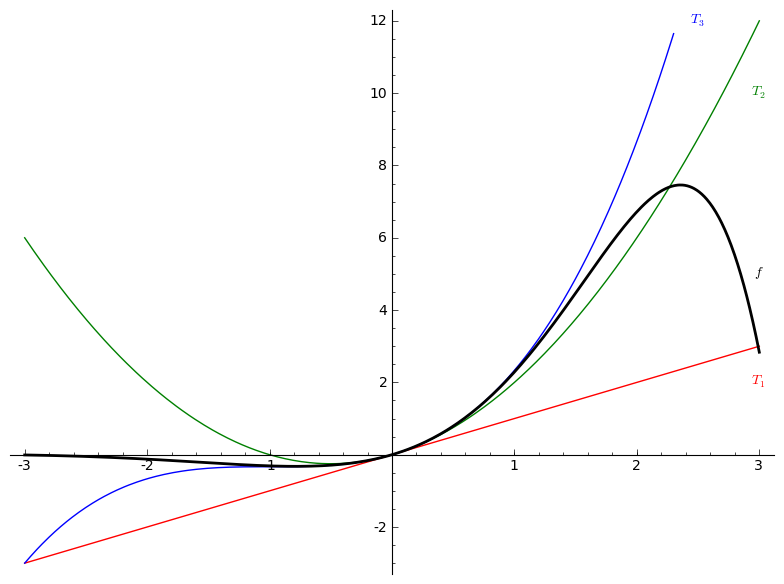
\includegraphics[scale=0.5]{figures/formel-taylor}
\end{center}

\end{frame}


\begin{frame}[fragile]


\evidence{Graphiques}

\begin{itemize}
  \item Courbe de Lissajous d'équation $t \mapsto \big(\cos(3t),\sin(4t)\big)$
  \uncover<2->{
  \item \codeinline{parametric_plot((cos(3*t),sin(4*t)),(t,0,2*pi))}
  }
  \uncover<3->{
  \item Graphe de la fonction $f(x,y)= \cos(xy)$
  }
  \uncover<4->{
  \item \codeinline{plot3d(cos(x*y),(x,-4,4),(y,-4,4))}
  }
  \uncover<5->{
  \item Définir les variables utilisées : \codeinline{var('t')}
\ et \  \codeinline{var('x,y')}
}
  
\end{itemize}



\begin{center}
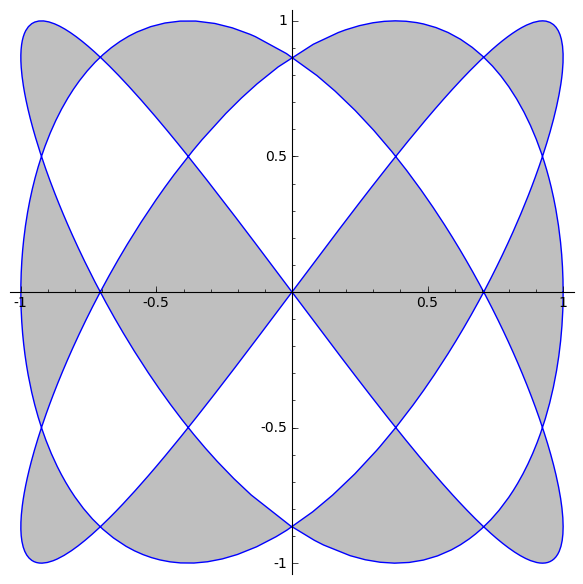
\includegraphics[scale=0.3]{figures/formel-lissajou}\ 
\uncover<3->{
\includegraphics[scale=0.18]{figures/formel-surface}
}
\end{center}
\end{frame}


%%%%%%%%%%%%%%%%%%%%%%%%%%%%%%%%%%%%%%%%%%%%%%%%%%%%%%%%%%%%%%%%
\section{Le calcul formel peut-il tout faire ?}

\begin{frame}[fragile]
\begin{tp}
\begin{enumerate}
  \item Pouvez-vous calculer les solutions réelles de $x^k-x-1=0$ pour les entiers $k \ge 2$ ?
  \item Est-ce que \Sage\ sait que toutes ces expressions sont nulles ?
  
  \vspace*{-4ex}
  $$2^{10} - 1024 \qquad (x+1)^2-x^2-2x-1 \qquad \sin^2(x)+\cos^2(x) - 1$$
\end{enumerate}  
\end{tp}

\pause

\begin{enumerate}
\item 
  \begin{itemize}
    \item \codeinline{solve(x^2-x-1==0,x)} renvoie deux solutions
$\frac{1+\sqrt5}{2}$ et $\frac{1-\sqrt5}{2}$
\pause
    \item \codeinline{solve(x^5-x-1==0,x)} renvoie seulement l'équation !
  \end{itemize}

\pause

\item 

\begin{itemize}
    \item \codeinline{2^10-1024} renvoie $0$ 
    \pause

    \item \codeinline{expand((x+1)^2-x^2-2*x-1)} renvoie $0$ 
    \pause

    \item 
    \codeinline{f = sin(x)^2+cos(x)^2 - 1} 
    
    \pause
    \codeinline{f.simplify_trig()} simplification pour obtenir $0$
  \end{itemize}


\end{enumerate}

\end{frame}



%%%%%%%%%%%%%%%%%%%%%%%%%%%%%%%%%%%%%%%%%%%%%%%%%%%%%%%%%%%%%%%%
\section{Un peu plus sur \Sage}

\begin{frame}[fragile]


\evidence{Syntaxe de \Sage}
\medskip

\pause
\begin{algo}[motiv-calcul-formel.sage (2)]
\begin{lstlisting}
for n in range(8):
    print n, factor(2^(2^n)+1)
\end{lstlisting}
\end{algo}

\pause
\begin{itemize}
  \item \codeinline{for n in range(N):} 
  
  $n$ parcourt les entiers de $0$ à   $N-1$
  
  \medskip 
  \pause 
  
  \item \codeinline{print n, factor(2^(2^n)+1)}
  
  est exécuté pour $n=0,1,\ldots,N-1$
  
  \medskip
  \pause
 \item L'indentation délimite les blocs d'instructions
\end{itemize}

\end{frame}



\end{document}
